%!TEX root = Thesis_David_Burns.tex
%ergh maybe just cut the shit out of this, we are just going to focus on a simple constant release anyway to start

\chapter{DMS Climatology Modelling}
\label{ch:dmsclim}

The way in which \gls{dms} is created and enters the atmosphere needs to be considered when attempting to model its effects on climate. There are a number of ways in which this can be treated: using large data maps, modelling the ocean, and/or applying different methods for ocean surface-to-atmosphere exchange (surface flux) \citep{woodhouse:2010ed}. These climatological models of \gls{dms} are needed to produce the chemical concentration maps used as input for any chemical transport model (see \cref{subsec:ctm}).

	\section{Modelling DMS production}
	\label{sec:modeldms}

	A number of studies exist for modelling \gls{dms}. Their methods provide guidance for which modelling systems are successful, and which \gls{dms} climatological models are necessary to produce realistic results.

	The Pacific Atmospheric Sulfur Experiment (\gls{pase}) measured \gls{dms} and \gls{sot} levels via flights made at \SI{40}{\metre} above sea level in the remote Pacific Ocean, near Christmas Island \citep{bandy2011pacific}. Other chemicals were also measured, including \gls{h2so4}. Using this data \citet{simpson:2014} devised budgets for \gls{dms}, \gls{sot} and \gls{nss} sulphate particles. The \gls{dms} budget consisted of surface flux, entrainment, oxidation and divergence. Using the budgets it was calculated that approximately \SI{20}{\percent} of \gls{dms} became \gls{nss} sulphate particles. 

	In the region measurements were taken from, an easterly jet stream from South America introduced \gls{nss} sulphate particles, originating from the land, into the \gls{mbl}. This was exacerbated by a localised subsidence. Modelling showed that the particles introduced via \gls{ft} entrainment dominated those produced from \gls{dms} for the region \citep{simpson:2014}. The study revealed that their results were influenced by regionally specific inputs that may not be present in the \gls{gbr}, and highlights the importance of localised modelling and the potential influence of particles from the \gls{ft} \citep{simpson:2014}.

	\citet{woodhouse:2010ed} produced a global model of \gls{dms} and its effects on \gls{ccn} concentration. Aerosol processes were modelled using \gls{glomapm} inside of a chemical transport model called TOMCAT. A number of \gls{dms} climatologies were tested, with the climatology developed by \citet{Kettle:2000jy} as a reference point (see \cref{sec:dmssurf}). The model showed that \gls{dms}'s highest impact on \gls{ccn} was in the southern hemisphere (see \cref{fig:wooddmsccn}). Also, any region with large anthropogenic \gls{ccn} sources sees little impact from \gls{dms} \citep{woodhouse:2010ed}. Overall, the global impact of \gls{dms} on \gls{ccn} in the model was low. It was also found that changes to \gls{ccn} production from different climate change scenarios could not be distinguished from variances arising from using different climatology models.

	\begin{figure}[!htb]
	    \centering
	    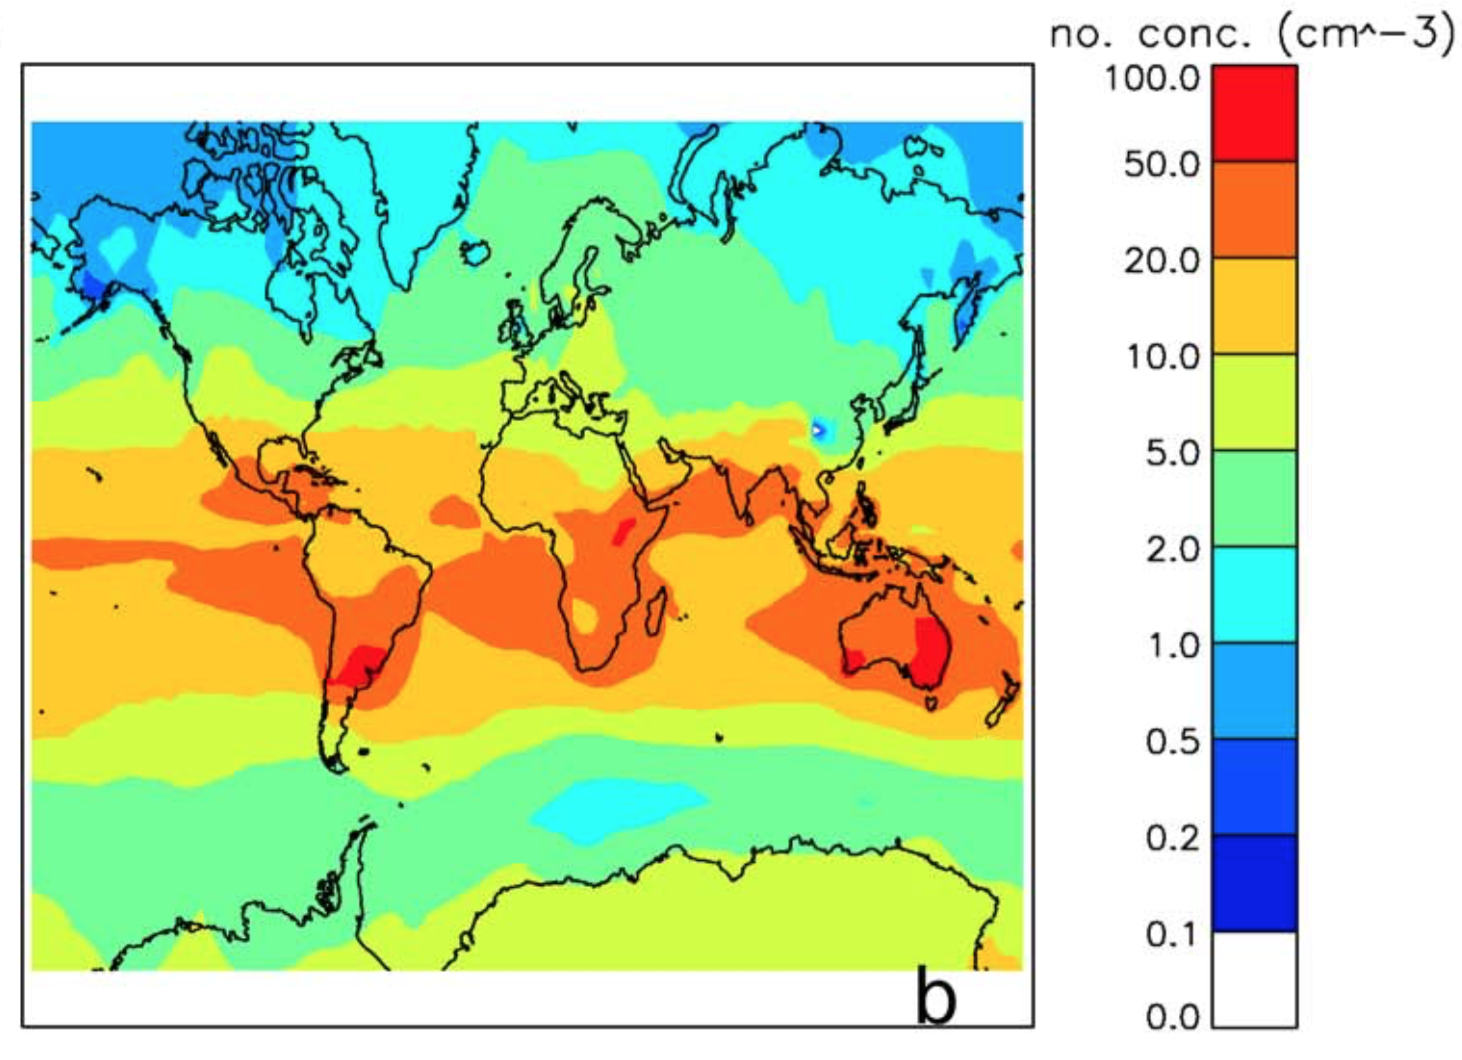
\includegraphics[width=0.6\textwidth,natwidth=1462,natheight=1060]{Fig/Literature_Review/wooddmsccn.png}
	    \caption{A global map of the difference between \gls{ccn} concentrations produced by model runs with and without \gls{dms} \citep{woodhouse:2010ed}.}
	    \label{fig:wooddmsccn}
	\end{figure}

	% What has been done around modelling in the southern hemisphere and the \gls{gbr} region specifically? Does this level of regionality matter in terms of modelling these processes?


%--------------------------------------------------------------------------------------------------------------------------%
%--------------------------------------------------------------------------------------------------------------------------%

	\section{DMS Surface Flux}
	\label{sec:dmssurf}

	As mentioned in \cref{subsec:ctm}, maps of the chemicals being analysed are required to feed into any chemical transport model used. For \gls{dms}, this is often given as a surface flux map for the region of interest. There are many meteorological and biological variables influencing \gls{dms} surface flux. The major meteorological variable is wind speed at the surface of the ocean \citep{Kettle:2000jy}. Surface concentrations of \gls{dms} are generally taken from experimental data with a flux model producing atmospheric concentrations \citep{woodhouse:2010ed}.

	\citet{Kettle:2000jy} describes a methodology for approximating a global \gls{dms} surface flux map. Data was collected from a large number of publications, study databases and direct correspondence with researchers (see \cref{fig:kettledata}). The data was then interpolated to provide monthly global \SI{1}{\degree} resolution sea surface \gls{dms} maps. Maps for sea surface salinity, temperature and chlorophyll concentration were also created \citep{kettle1999global}. In \citet{Kettle:2000jy} the surface concentration maps from \citet{kettle1999global} were converted to surface flux maps using a technique from \citet{liss:1983iu} The transfer rate was assumed to be a function of the concentration difference between the ocean and air, and the piston velocity, which depends on wind speed. Other surface flux methods were also examined and the differences between them produced an error in \gls{dms} results greater than \SI{50}{\percent}. Overall, the method showed little dependence on meteorological changes to \gls{dms} flux, around \SI{10}{\percent} for future predicted changes.

	\begin{figure}[!htb]
	    \centering
	    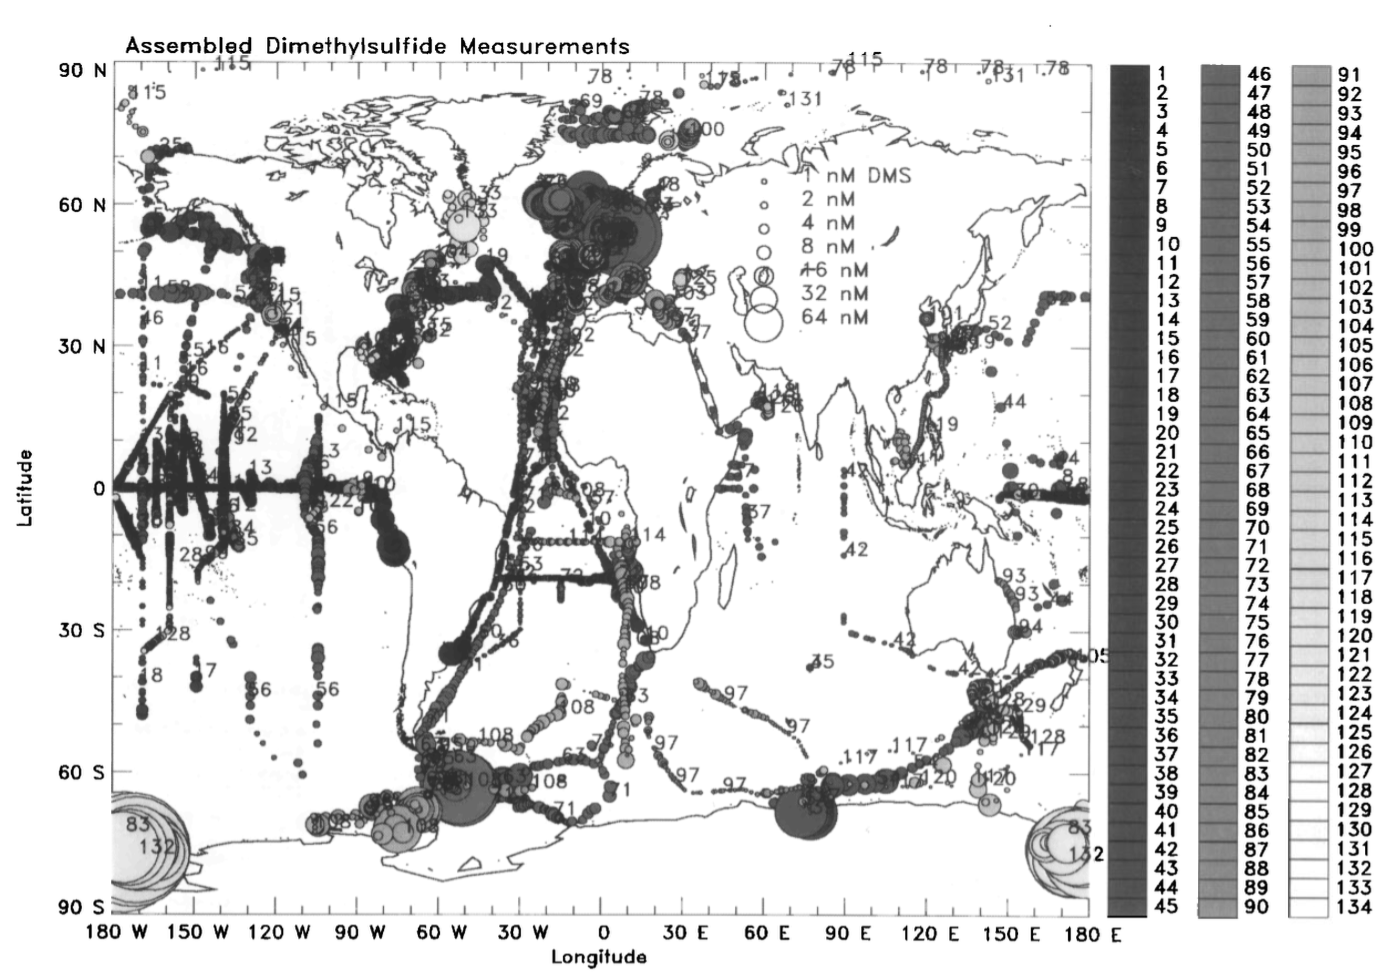
\includegraphics[width=0.8\textwidth,natwidth=1414,natheight=1344]{Fig/Literature_Review/kettledata.png}
	    \caption{The global measurement data used for producing interpolated maps of \gls{dms} sea surface concentrations \citep{kettle1999global}. Larger circles indicate higher concentrations while shading defines the contributor.}
	    \label{fig:kettledata}
	\end{figure}

	\citet{lana2011updated} expanded on this work producing a more complete and accurate climatological model of \gls{dms} surface flux. Their model indicates a summer increase in surface flux (see \cref{fig:lanadmsmaps}) and also a vertical dependence on atmospheric \gls{dms} concentration. The database of measurements used was also three times larger than that of \citet{kettle1999global}, resulting from continued efforts into the SOLAS project (Surface Ocean Lower Atmosphere Study) \citep{lana2011updated}.

	\begin{figure}[!htb]
	    \centering
	    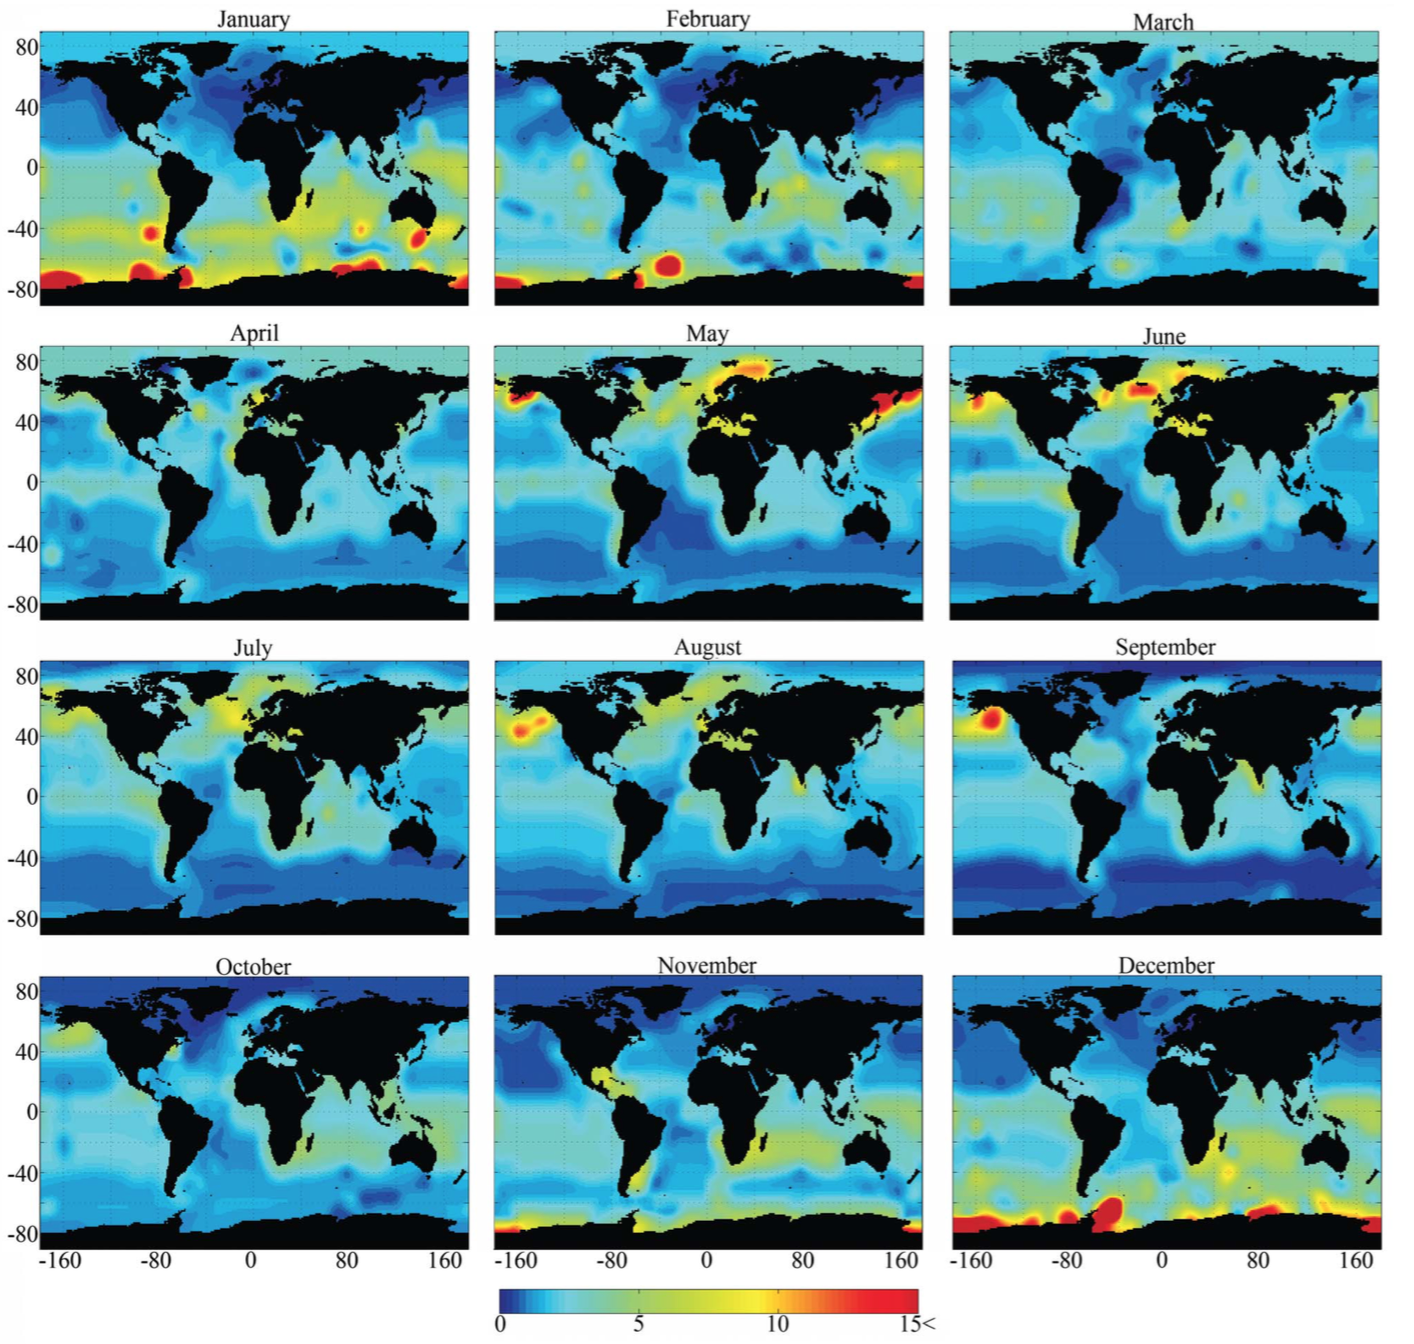
\includegraphics[width=0.9\textwidth,natwidth=1414,natheight=1344]{Fig/Literature_Review/lanadmsmaps.png}
	    \caption{Monthly global maps of \gls{dms} concentrations produced using surface concentrations and an updated surface flux parameterisation \citep{lana2011updated}. Increases in \gls{dms} concentrations during summer periods can be seen.}
	    \label{fig:lanadmsmaps}
	\end{figure}

	The observational data for the \gls{gbr} was largely sourced from \citet{jones:2005ez}. Interestingly, both ocean surface and atmospheric \gls{dms} concentrations were measured in this study. The significance of a regional and diurnal dependence on \gls{dms} concentrations indicates that the global results obtained in \citet{lana2011updated} should not be assumed for regionally specific models.



	% What methods are around for estimating the flux?
	% constant, kettle, nightingale, lana
	% kettle describes a large collection of sea surface dms concentrations which is then interpolated to cover the entire globe, 
	% how are these papers tied together? what does each do individually?
	% what are the actual functions that relate sea surface concentraions to atmos concentrations?

	% Is Jones data for the \gls{gbr} used in these inventories? 'some early data was'

	% What effect does changing climate and meteorology have on these fluxes?
	% Globally wind speed is the dominant process.
	% There may be some correlations found in the local \gls{gbr} region that could be used to form some time and met dependent source functions. 'need to explore some of jones papers for this'. This is about the tide link found in jones paper.


	% Has anyone actually made surface concentration measurements at the \gls{gbr}?
	% What does Graham Jones have to say about this? Has he replied to your email?




%--------------------------------------------------------------------------------------------------------------------------%

		% \subsection{Kettle et al.}
		% \label{subsec:kettle}

		% The Kettle paper is a treasure trove of old DMS surface concentration papers. There are hundreds of sources in the introduction and it seems to be really complete. Of course the paper itself is over 15 years old now.

		% Supposedly there is a database available of dms concentrations from geia... I couldn't find it, but maybe it's there. Kettle mentions it.

		% They used a method similar to other well established global emission maps. A large quantity of experimental data was collected from publications and directly from scientists. This included DMS surface concentrations along with a number of other values like ocean height, temperature 'put actual list here'. 

		% The estimates of the error produced in this paper may not encompass errors associated with coral reef production of DMS. They use some strange method for producing the approximated error that I don't understand too well. However they use a comparison with chlorophyll which is not necessarily a good indicator for coral reef produced DMS. Does the coral or it's symbiot even have the type of chlorophyl Kettle uses?

		% There is very little correlation between their DMS map and other maps of various climatological measures. The highest was surface temperature, then chlorophyll a concentration.

		% They have split the world map up into sections, one of which is AUSE, the east coast of Australia. From the figures it appears to be almost constant spatially and temporally. This doesn't seem to match the variability of measurements taken by Jones et al.

		% It might be a good idea to include one of the global map images that is in the Kettle paper. It gives a good idea of what the method actually is. Probably the one on 434.

		% "Smoothed maps must be viewed skeptically because the data assimilation scheme was based mostly on modeled and extrapolated data and should therefore be corroborated with more measurements. Still, the scheme illustrates the kind of fields which could be generated with a larger database of observation." from Kettle. Has there been another attempt at this with newer databases?

		% I don't really get what the big deal is with this paper. It doesn't really provide a usable map. They collected a database of experimental data, mapped it to a globe and then used some smoothing functions. I would need to get the data they used to do anything, and anyway, they haven't really outlined very well the sorts of mathematical techniques they used for their smoothing. They mention a few papers along the way that I should probably look at that are meant to talk about the approximating techniques used.

		% I think perhaps the idea of the paper is that you are meant to get the latest data on DMS measurements and then follow their smoothing and approximation techniques.


%--------------------------------------------------------------------------------------------------------------------------%
%--------------------------------------------------------------------------------------------------------------------------%

	% \section{DMS Surface Flux Paramterisations}

	% what is this about?

	% what different methods are there for defining these parameters?

	% what sort of variability arises from this?

	% talk about the frankly insane levels of varioability from these different methods. What does this mean for any model that makes use of them?

	% nightingale and lana?
	% % 		what are the actual functions that relate sea surface concentraions to atmos concentrations?



% 'i think dump these subsections and keep them to a paragraph explaining the progressions of dms climatological modeling'
%--------------------------------------------------------------------------------------------------------------------------%

% 		'do we need a section here specifically for taking ocean dms concentrations and turning them into atmos concentrations?'
% 		\subsection{Nightingale}

% 		what are the actual functions that relate sea surface concentraions to atmos concentrations?




% %--------------------------------------------------------------------------------------------------------------------------%

% 		\subsection{Lana}




%--------------------------------------------------------------------------------------------------------------------------%
%--------------------------------------------------------------------------------------------------------------------------%

	% \section{Mechanistic Model of DMS surface concentrations}

	% why is this important? what benefits are there over observations?

	% what are some?

	% how do they compare to the interp fields?

	% how do they compare to observations, both regional and global?

	% Is there anything specific to the great barrier reef? Or even to any reef system?

	% Why cant we just apply one of the existing models to the \gls{gbr}?

	% 'from woodhouse 2010'
	% However, for studies of multi-annual variability, long term trends and climate feedbacks it is necessary to develop a mechanistic model or parameterisation of DMS production and concen- tration on a global scale. These diagnostic models require evaluation, and one way to do that is to compare them di- rectly against point observations or the interpolated fields of, for example, Kettle and Andreae (2000). Boucher et al. (2003) compared the Kettle and Andreae (2000) observa- tional climatology, the Belviso et al. (2004b) climatology from SeaWiFS satellite chlorophyll, and the model derived climatology of Aumont et al. (2002), in an atmospheric general circulation model (GCM). The three different DMS sources produced only a small range of calculated global DMS flux of between 24 and 27 Tg a−1 sulphur, but with large differences in spatial distribution. Belviso et al. (2004a) examined the differences between seven climatologies: the two observational climatologies of Kettle et al. (1999) and Kettle and Andreae (2000); the light, nutrients and chloro- phyll relationship of Anderson et al. (2001), the Simo ́ and Dachs (2002) mixed layer depth (MLD) and chlorophyll-a relationship; the Belviso et al. (2004b) and Aumont et al. (2002) relationships noted above; and a process model de- scribed in Chu et al. (2003). They concluded that there are locally up to 100\% differences in DMS seawater concentra- tion, particularly at high latitudes, and that none of the clima- tologies provides a complete representation of oceanic DMS concentrations. The impact of the different climatologies on sea-air fluxes and sulphate aerosol was not calculated.

